\documentclass[10pt,a4paper]{article}
\usepackage[margin=.78in]{geometry}\usepackage[T1]{fontenc}
\usepackage{lmodern,microtype,booktabs,tabularx,graphicx,xcolor,hyperref}
\hypersetup{hidelinks}\setlength{\parindent}{0pt}\setlength{\parskip}{6pt}
\title{IDM-Viz: External Split and Model Sensitivity on UCI 224}
\author{Ahmed Bilal (23I-2581) \and Umar Behram (23I-2604)}\date{16 November 2026}
\begin{document}\maketitle
\begin{abstract}
We tested whether external cohort results depended on one historical partition or the frozen logistic classifier. Six stratified historical splits, two models and one- versus two-cohort history windows were scored on shared UCI acquisition batches 3--10. Calibrated correctness transfer remained poor and varied materially by model/window. These repeated splits are sensitivity analyses on one dataset, not independent replications or evidence of general transfer.
\end{abstract}
\section{Locked extension}
We used UCI Gas Sensor Array Drift with six states (420001--420006), a 60/20/20 train/calibration/reference split, logistic regression and a fixed depth-6 decision tree. The one-cohort history uses batch 1; the pooled history uses batches 1--2. The latter has a larger training and labelled history budget. To compare windows fairly, reported cross-window metrics use the shared later batches 3--10; batch 2 is shown separately in raw result tables. All transformations and correctness calibrators use historical training/calibration data only. Monitoring labels appear only in evaluator outputs.
\section{Results}
\begin{table}[ht]\centering\small
\caption{Mean and standard deviation across six random historical splits, averaged equally over shared cohorts 3--10. Split variation is descriptive.}
\begin{tabular}{llrrrrr}\toprule History & Model & Accuracy & Macro-F1 & Calibrated MAE & Raw-confidence MAE & Reference-accuracy MAE \\\midrule
Batch 1 & Logistic & 0.423 $\pm$ 0.025 & 0.279 $\pm$ 0.024 & 0.553 $\pm$ 0.019 & 0.428 & 0.534 \\
Batch 1 & Depth-6 tree & 0.410 $\pm$ 0.015 & 0.303 $\pm$ 0.015 & 0.374 $\pm$ 0.050 & 0.426 & 0.399 \\
Batches 1--2 & Logistic & 0.645 $\pm$ 0.031 & 0.560 $\pm$ 0.032 & 0.342 $\pm$ 0.033 & 0.173 & 0.342 \\
Batches 1--2 & Depth-6 tree & 0.528 $\pm$ 0.007 & 0.434 $\pm$ 0.004 & 0.401 $\pm$ 0.013 & 0.358 & 0.408 \\
\bottomrule\end{tabular}\end{table}
For batch-1-only history, calibrated accuracy-estimate MAE was 0.553 for logistic regression and 0.374 for the tree. With batches 1--2 pooled, it was 0.342 for logistic and 0.401 for the tree. The extra history changes the task and label budget, so these differences are not a causal estimate of the value of adding batch 2. Raw confidence was the strongest reported estimator for batch-1 logistic in the shared-window comparison (MAE 0.428), while the calibrated tree was best among the displayed estimates at MAE 0.374. No one estimator dominates across these configurations.
\begin{figure}[ht]\centering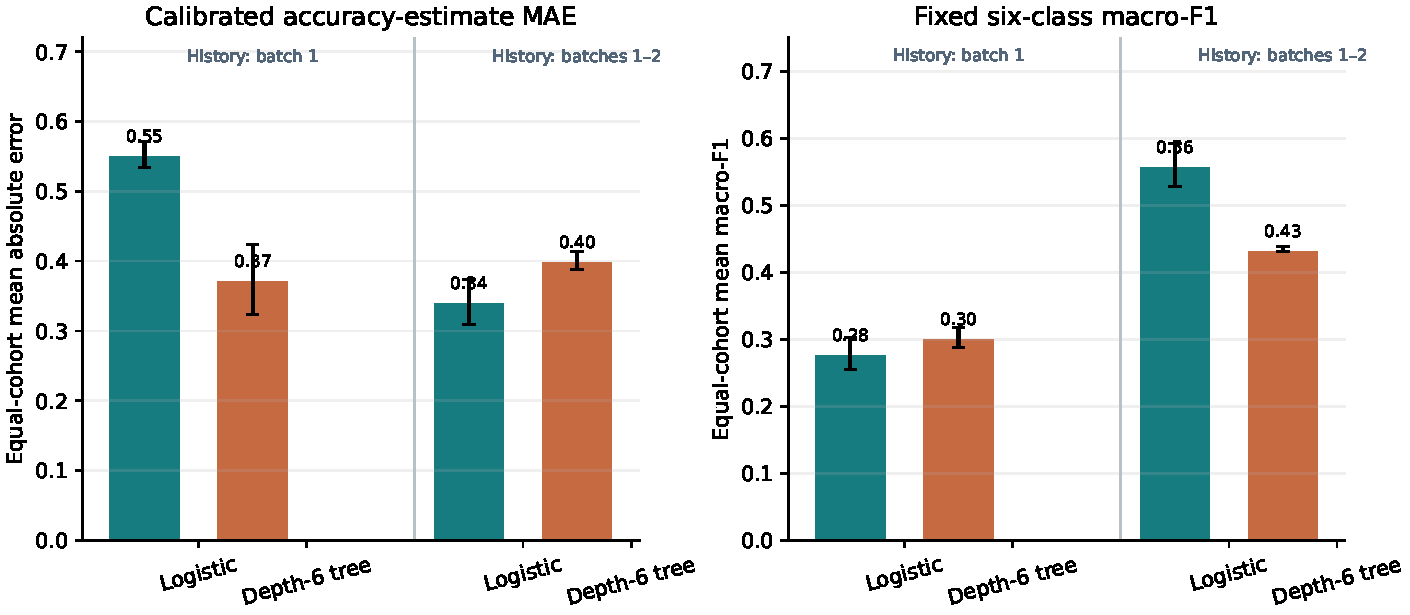
\includegraphics[width=.96\linewidth]{split_model_sensitivity.pdf}
\caption{Mean performance and calibrated-estimate error by model and history window. Error bars show standard deviation across six random splits, not confidence intervals over datasets.}
\end{figure}
\section{Scope and limitations}
This extension tests sensitivity to split and learner choice, not temporal adaptation or multiple-domain generalization. Splits overlap the same underlying records; six split seeds are not six independent datasets. The pooled-history window has more labelled history. The calibration transfer errors remain substantial and do not justify an all-purpose accuracy estimate under conditional shift. No interval guarantee or harmful-shift certainty follows from these metrics. The original Phase 2 DOCX and primary external outputs are unchanged.
\section{Reproduction}
\begin{verbatim}
python scripts/run_uci224_split_model_sensitivity.py --out results/phase3/uci224_NEW
python scripts/evaluate_uci224_split_model_sensitivity.py --run results/phase3/uci224_NEW
python scripts/report_uci224_split_model_sensitivity.py
\end{verbatim}
\end{document}
